% \documentclass[runningheads]{llncs}
\documentclass[11pt]{article}
%\usepackage[utf8]{inputenc}

\usepackage{graphicx}
\usepackage{amsmath}
\usepackage{amssymb}
\usepackage{arydshln}
\usepackage{xcolor,ulem}

\usepackage{wrapfig}

% Used for displaying a sample figure. If possible, figure files should
% be included in EPS format.
%
% If you use the hyperref package, please uncomment the following line
% to display URLs in blue roman font according to Springer's eBook style:
% \renewcommand\UrlFont{\color{blue}\rmfamily}

\setlength{\parskip}{0cm}
\setlength{\parindent}{1em} 

\addtolength{\oddsidemargin}{-.875in}
\addtolength{\evensidemargin}{-.875in}
\addtolength{\textwidth}{1.75in}

\addtolength{\topmargin}{-.875in}
\addtolength{\textheight}{1.75in}


\newcommand{\reals}{\mathbb{R}}

\newcommand{\comment}[3]{{\color{#1} {\bf #2 :} #3}}
%\newcommand{\comment}[3]{}  % suppress comments
% Use these macros to make comments.
\newcommand{\kui}[1]{\comment{blue}{Kui}{#1}}
\newcommand{\yoav}[1]{\comment{purple}{Yoav}{#1}}
\renewcommand{\beth}[1]{\comment{red}{Beth}{#1}}
\newcommand{\david}[1]{\comment{cyan}{David}{#1}}
\newcommand{\zhongkai}[1]{\comment{brown}{Zhongkai}{#1}}

\renewcommand\floatpagefraction{.99}
\renewcommand\topfraction{.99}
\renewcommand\bottomfraction{.99}
\renewcommand\textfraction{.1}

\setcounter{totalnumber}{50}
\setcounter{topnumber}{50}
\setcounter{bottomnumber}{50}
\setlength{\abovecaptionskip}{0pt}
\setlength{\belowcaptionskip}{0pt}

\title{Towards explainable computer assisted Neuroanatomy}
\author{Kui Qian, Zhongkai Wu, Beth Friedman, David Kleinfeld, Yoav Freund}
\date{August 2022}

\begin{document}

\maketitle

\begin{abstract}
  A fundamental goal of neuroanatomy is the annotation of cells and
  structures.  Manual annotation of structures is based on the spatial
  distribution of cell shape, size, orientation and density.  New
  technology is enabling the rapid imaging of entire brains at high
  resolution. However, manual identification of structures in these massive datasets, as well as the molecular labeling cells based on
  specific patterns of genetic expression,  is prohibitively
  time consuming.  We present a machine
  learning methodology for developing digital assistants that
  significantly reduce the labor of the anatomist while improving the
  consistency of the annotation.

  Our methodology is based on designing, for each annotation problem,
  a large number of features and using boosting on manually annotated
  images to select the most predictive features. We describe two annotation tasks to which we applied this approach. The first, more complex task is detecting specific structures in the brainstem of the mouse. The second is the detection of individual cells marked by a fluorescent indicator. We provide the details of both of these applications and show that they significantly reduce the anatomist's labor in completing these tasks.
  
  %We translate each cell image into a feature vector that
  %includes aspect ratio, orientation and area, as well as additional
  %features derived using a graph Laplacian. The algorithm uses thehttps://www.overleaf.com/project/626c35fc11c79a37dffd2ffc
  %statistical distribution of these features vectors to identify brain
  %structures.
\end{abstract}

\section{Main}
We propose a system for detecting anatomical structures in the mouse
brain. Our system takes as input high-resolution images of aligned
sections. It produces as output the estimated center of mass (COM) for
each structure. Each detection is assigned a confidence. High
confidence structures are associated with a visual explanation.

\subsubsection {Significance for Neuroscience}

%\yoav{I would start with something intended to a broader audience, with little or no familiarity with sections/stains/structures, and say what is the significance *of* neuroanatomy, before saying what the significance of our methods *for* neuroanatomy. Something along the lines of: Big data technology for neuroscience has been advancing by leaps and boundsover the past decades. It is now possible to simultanuously record the activity of XXX neurons, use mathilation tags (?) to identify different types of neurons...
How do we study the computational power of brains? Brains are composed of circuits that have multiple scales of organization, the microscopic-scale of connections between neurons, i.e., one to ten micrometers, the mesoscopic-scale of collections of neurons with similar functionality, i.e., hundred of micrometers to millimeters. Molecular  tagging of neuronal cell types by the expression of genetically encoded reporters and light-level imaging of the cells and tags, using both transmission and fluorescent microscopy, plays an essential role in this process. The resulting raw data files are extremely large, from 1 to 100 TB per rodent brain. The current means for quantification and spatial mapping of tagged neuronal populations in brain sections require labor intensive annotation by expert neuroanatomists. How can machine learning assist with this process and minimize the amount of manual work involved while maintaining accuracy and consistency.

%Further, how can machine learning assist neuroscientists is to combine experimental results from the brains of different animals.

%Neuroanatomical observations depend on mapping data from images, obtained as consecutive planar sections, to reference brains.
%This presents a number of challenges. In many cases the individual sections may carry distortions, and further need to be aligned to form a three-dimensional representation of a brain. The second challenge is the identification of brain structures. Classically, this relies on the use of a stain, i.e., a labels that marks a restricted part of the brain cells and allows both individual cells and clusters of like cells to be identified. This is an art form
% \yoav{ Instead of "art form" I would say "requires significant expertise and many hours of work". I would also say something about the need to create work-flows that combine less expert annotators (Julian and Marissa) and more expert annotators (Beth) to achieve the required throughput with sufficient accuracy.} , as different stains highlight different organelles of brain cells and different sectioning techniques reveal yield seemhttps://www.overleaf.com/project/626c35fc11c79a37dffd2ffcingly different textures in the organization of neurons. Currently, human scanning is used to find the best match of a given structure, from the subject brain, to an annotated reference brain atlas. This match to sample approach does not readily support assessment of observational differences between laboratories nor provide a means for assessing and compensating for common systematic errors.
% Critically, human observers do not provide a path toward either understanding of critical features that define a structure nor a means toward automation.
% \yoav{ I don't understand the last sentence. In my mind, it is a question of resources. My assumption is that the "ground truth" is achievable by an expert anatomist spending sufficient time. What we are attempting to do is (1) save anatomist time (2) allow less expert anatomist to do the task (3) provide meaningful confidence levels and (4) provide explanations for the confident predictions.}

Machine learning methods, mostly based on Neural Network (NN), have been used to automate brain section analysis~\cite{}. However, as NN models are black boxes that define input-output relationships, the models provide no insight as to how decision are made. Nor do NNs give a measure of confidence. It is thus very hard for a neuroanatomist to understand {\em why} the NN made particular decisions. In this paper we present an alternative approach with models that operate in a way more similar to the neuroanatomist and that generates outputs which the neuroanatomist can interpret and correct.

The models generated by the methods described in this paper have three advantages over models generated. First, the basic units of analysis are cells, not pixels. Second, a confidence level is computed for each detection, based on an ensemble of models. Finally, confident detections are associated with a visual explanation that can be used as feedback to the neuroanatomist.

The goal of the first method is to assist in the detection of tagged cells. The model is designed to report two confidence levels, i.e., sure and unsure. The anatomist need only sample the sures for quality assurance and label any false positives.  In contrast, the anatomist needs to check every unsure, yet this population is relatively small so that, overall, the methods provides a substantial savings in time.

The goal of the second method is to localize brain structures, such as motor or premotor nuclei in the brainstem. We focus on centroids to provide objective sign posts for rapid human verification of brain structure position. Our models make use of cell shape, orientation, density as well as more abstract quantities and boundaries of the structures. In addition to the three dimensional location of each structure, the model generates a meassure of confidence to offsets in any direction. In addition, the model generates a visual explanation for the localization in terms of cell features.

% Manual neuroanatomical analysis of brain sections is critical for creating accurate quantitative results. On the other hand, performing neuroanatomical analysis is expensive as it requires many hours of work of an expert anatomist.

% We consider two labor intensive tasks. Localizing anatomical structure and counting marked cells. Both tasks involve identifying and marking locations in images and both require expertise.

\subsubsection{Our data sets}

We use mouse brains that are serially sectioned and counterstained with one fluorescent tag to reveal all brain cells.  In addition, specific cell types are labeled with a second, different fluorescent tag. This results in a dual tagging approach where all cells are labeled by an inexpensive counterstain and a subset of interest is labeled by a second experimentally incorporated fluorophore. This has the advantage of narrowing the population of false detections as labeled neurons undergo a two-factor authentication scheme. 


\subsubsection{Our approach}

\yoav{This is currently only about marked cells, there is more to say about structure detection. I would include: cell-based analysis, confidence quantification and detection explanation.}
An important observation on locating both structures and cells is that while a typical section will contain hard to identify features and locations, most of the identifications are easy. This observation leads to the following approach to automation. We
use so-called {\em confidence rated detectors}. These detectors
associate with each detection a confidence score. A high confidence
score implies that the example is ``easy''  while the rest are
``hard''. This reduces the workload on the anatomist to the following
tasks:
\begin{itemize}
  \item {\bf Confirming the confident detections} In this step the
    anatomist recieves a small sample of the confident detections and
    verifies that they are correct. The sample size depends on the
    desired accuracy.
    \item {\bf classifiying the unconfident detections} In this step
      the anatomist labels {\em all} of the low confident predictions.
    \item {\bf searching for misses:} In this step the anatomist looks
      for locations that were completely missed by te detector.
  \end{itemize}
  
\subsubsection{Assistive AI} Traditionally, the goal of artificial
  intelligence is to design algorithms which mimic human behavior. AI
  systems are expected to perform as well as humans and, eventually,
  better than humans.

Indeed, in some domains, such as the game of go \cite{silver2017mastering} deep neural
networks (DNN)  have achieved super-human capabilities. In addition,
on highly curated image classification datasets such as ImageNet~\cite{deng2009imagenet} and
CIFAR~\cite{krizhevsky2009learning} DNNs give performance that, some argue, is better than
human. 

However, DNNs have some fundamental drawbacks that limit their
applicability to real-world problems. One problem is that DNNs
require large amounts of training data.
In some setups, such as alpha-go, the labels are generated automatically as
the program plays against itself. However often labels are generated by a
human expert and collecting large amounts of data is
prohibitively expensive. This is the case in the context of this
paper, where each labeled example corresponds to the 3D location of a
cell or a structure.

A second problem is that the training data and the test data are assumed to
come from the same distribution. However, in most real-world
applications the test data is drawn after the training is complete and
is often generated by a setup that is different from the one used to
collect the training data.
Specifically, in brain imaging, two brain section images from the same
location in different brains are likely to look quite differently.
These images vary for a variety of reasons including: animal to animal variability,
variability in the preparation process, including staining,
sectioning and imaging. In order to create robust classifiers, that do
not need to be retrained on each brain, we need a learning algorithm
that identifies robust patterns that are preserved across brains.
identifies patterns that are consistent across brains.

A third problem arises from variability in human labeling. We use
the term {\em inter raters variation} to refer to the difference in
labels between anatomists. We use the term {\em intra rater
  variation} to refer to the difference in the labels generated by the
same anatomist at different times. Inter and intra rater variations
have been studied in medicine~\cite{gellhorn2013inter}. One
contribution of this paper is an evaluation of rater variation in
neuroanatomy and it's relation to the {\em confident/un-confident}
classifications generated by our methods.

\subsubsection{Boosting and sparse representations}
An important part of the design of any learning algorithm is finding a
representation of input feature vectors that captures the aspects that are
most relevant for the classification task. In some situations deep
neural networks can find internal representations autonomously,
without human intervension. However, a close look at the design of
alpha-Go~\cite{silver2017mastering} reveals the high level of human
expertise used to design the features used by the NN.

Boosting~\cite{FreundSc97,schapire2013boosting} is another popular
learning algorithm which combines a large number of so-called ``weak''
rules to construct a single ``strong'' rule. Here we follow an
approach to feature detection for boosting that can be described as
{\em the kitchen sink approach}. This approach starts by the human
constructing a very large number of candidate rules. The boosting
algorithm performs both {\em feature selection} i.e. finding the rules
that provide significant information about the label. As well as feature weighting and
combination, i.e. finding how to combine the informative features to
predict the label.\footnote{Popular boosting software, such as XGBoost and
  LightGBM, use decision trees to combine the features.}

In general, increasing the number of features or rules increases the
danger of over-fitting. However, as shown in ~\cite{SchapireFrBaLe98}, the
number of features has only a small influence on overfitting. rather,
it was shown, that the distribtuion of the large {\em normalized
  margin} guarantees low overfitting even if the number of features
goes to infinity.


\subsubsection{Boosting and object detection}
The original Adaboost algorithm is designed for the problem of binary
classification. On the other hand, the problems we attack in this
paper are those of {\em object detection} where the object to be
detected is a structure or a marked cell.

In~\cite{violajones01} Viola and Jones demonstrated that boosting
achieves superior speed and accuracy in the task of face detection,
which is now a universal feature in smart phones and cameras.  The
approach used is the pospular {\em sliding-window} approach used in
many other system.  The input to the classifier consists of windows of
different sizes and locations in the image. At the training phase each
window is labeled +1 if it contains the object and 0 if is does
not. At test time the sliding window is used to generate inputs for
the detector and windows that that recieve a high score are defined to
be the predictions.

Viola and jones used so-called {\em Haar features} to represent the
features. The set of features is large ($\sim 10^5$) and was designed
specifically for objects where horizontal and vertical contrasts are
dominant, based on the assumption that faces in photos are usually
upright. This is an example of the {\em kitchen sink} approach where
many features are proposed, but only few are used in the final detector.

We use a very similar design to that of Viola and Jones. We use a 2D
detector to identify marked cells and a 3D detector to identify the 3D
location of a structure in a sectioned brain.

\subsubsection{Cell based analysis}

In~\cite{chen2019active} Chen et al used a sliding window and a
Neural network to detect brain structures. The window size is fixed at
$100 \mu m \times 100 \mu m$ which means that a typical window contains 10-100 cells.
The window is used as input to a pre-trained neural network which maps
each window to a vector of 1,000 features. The output layer of
this network is trained using logistic regression. The earlier layers
are fixed. Chen et al used this system to demonstrate the first
structure detection that operates at the resolution of single cells.
However, the concept of a cell is not directly used by this as the
input to the neural network consists of raw pixel values, and not any
higher-order features.

On the other hand, anatomist base their analysis on cytoarchitecture,
which, in turn, is based on the shapes of individual cells and the
relationshp between them. This makes it harder for the anatomist to
understand the decisions of the detector.

To remedy this problem and make the detections explainable, we use
features that are based on the shapes of individual cells.

\section{Results}

We present results from two detection systems. The first is for detecting known
brain structures. The second is for detecting marked cells. 

\begin{figure}[t]
  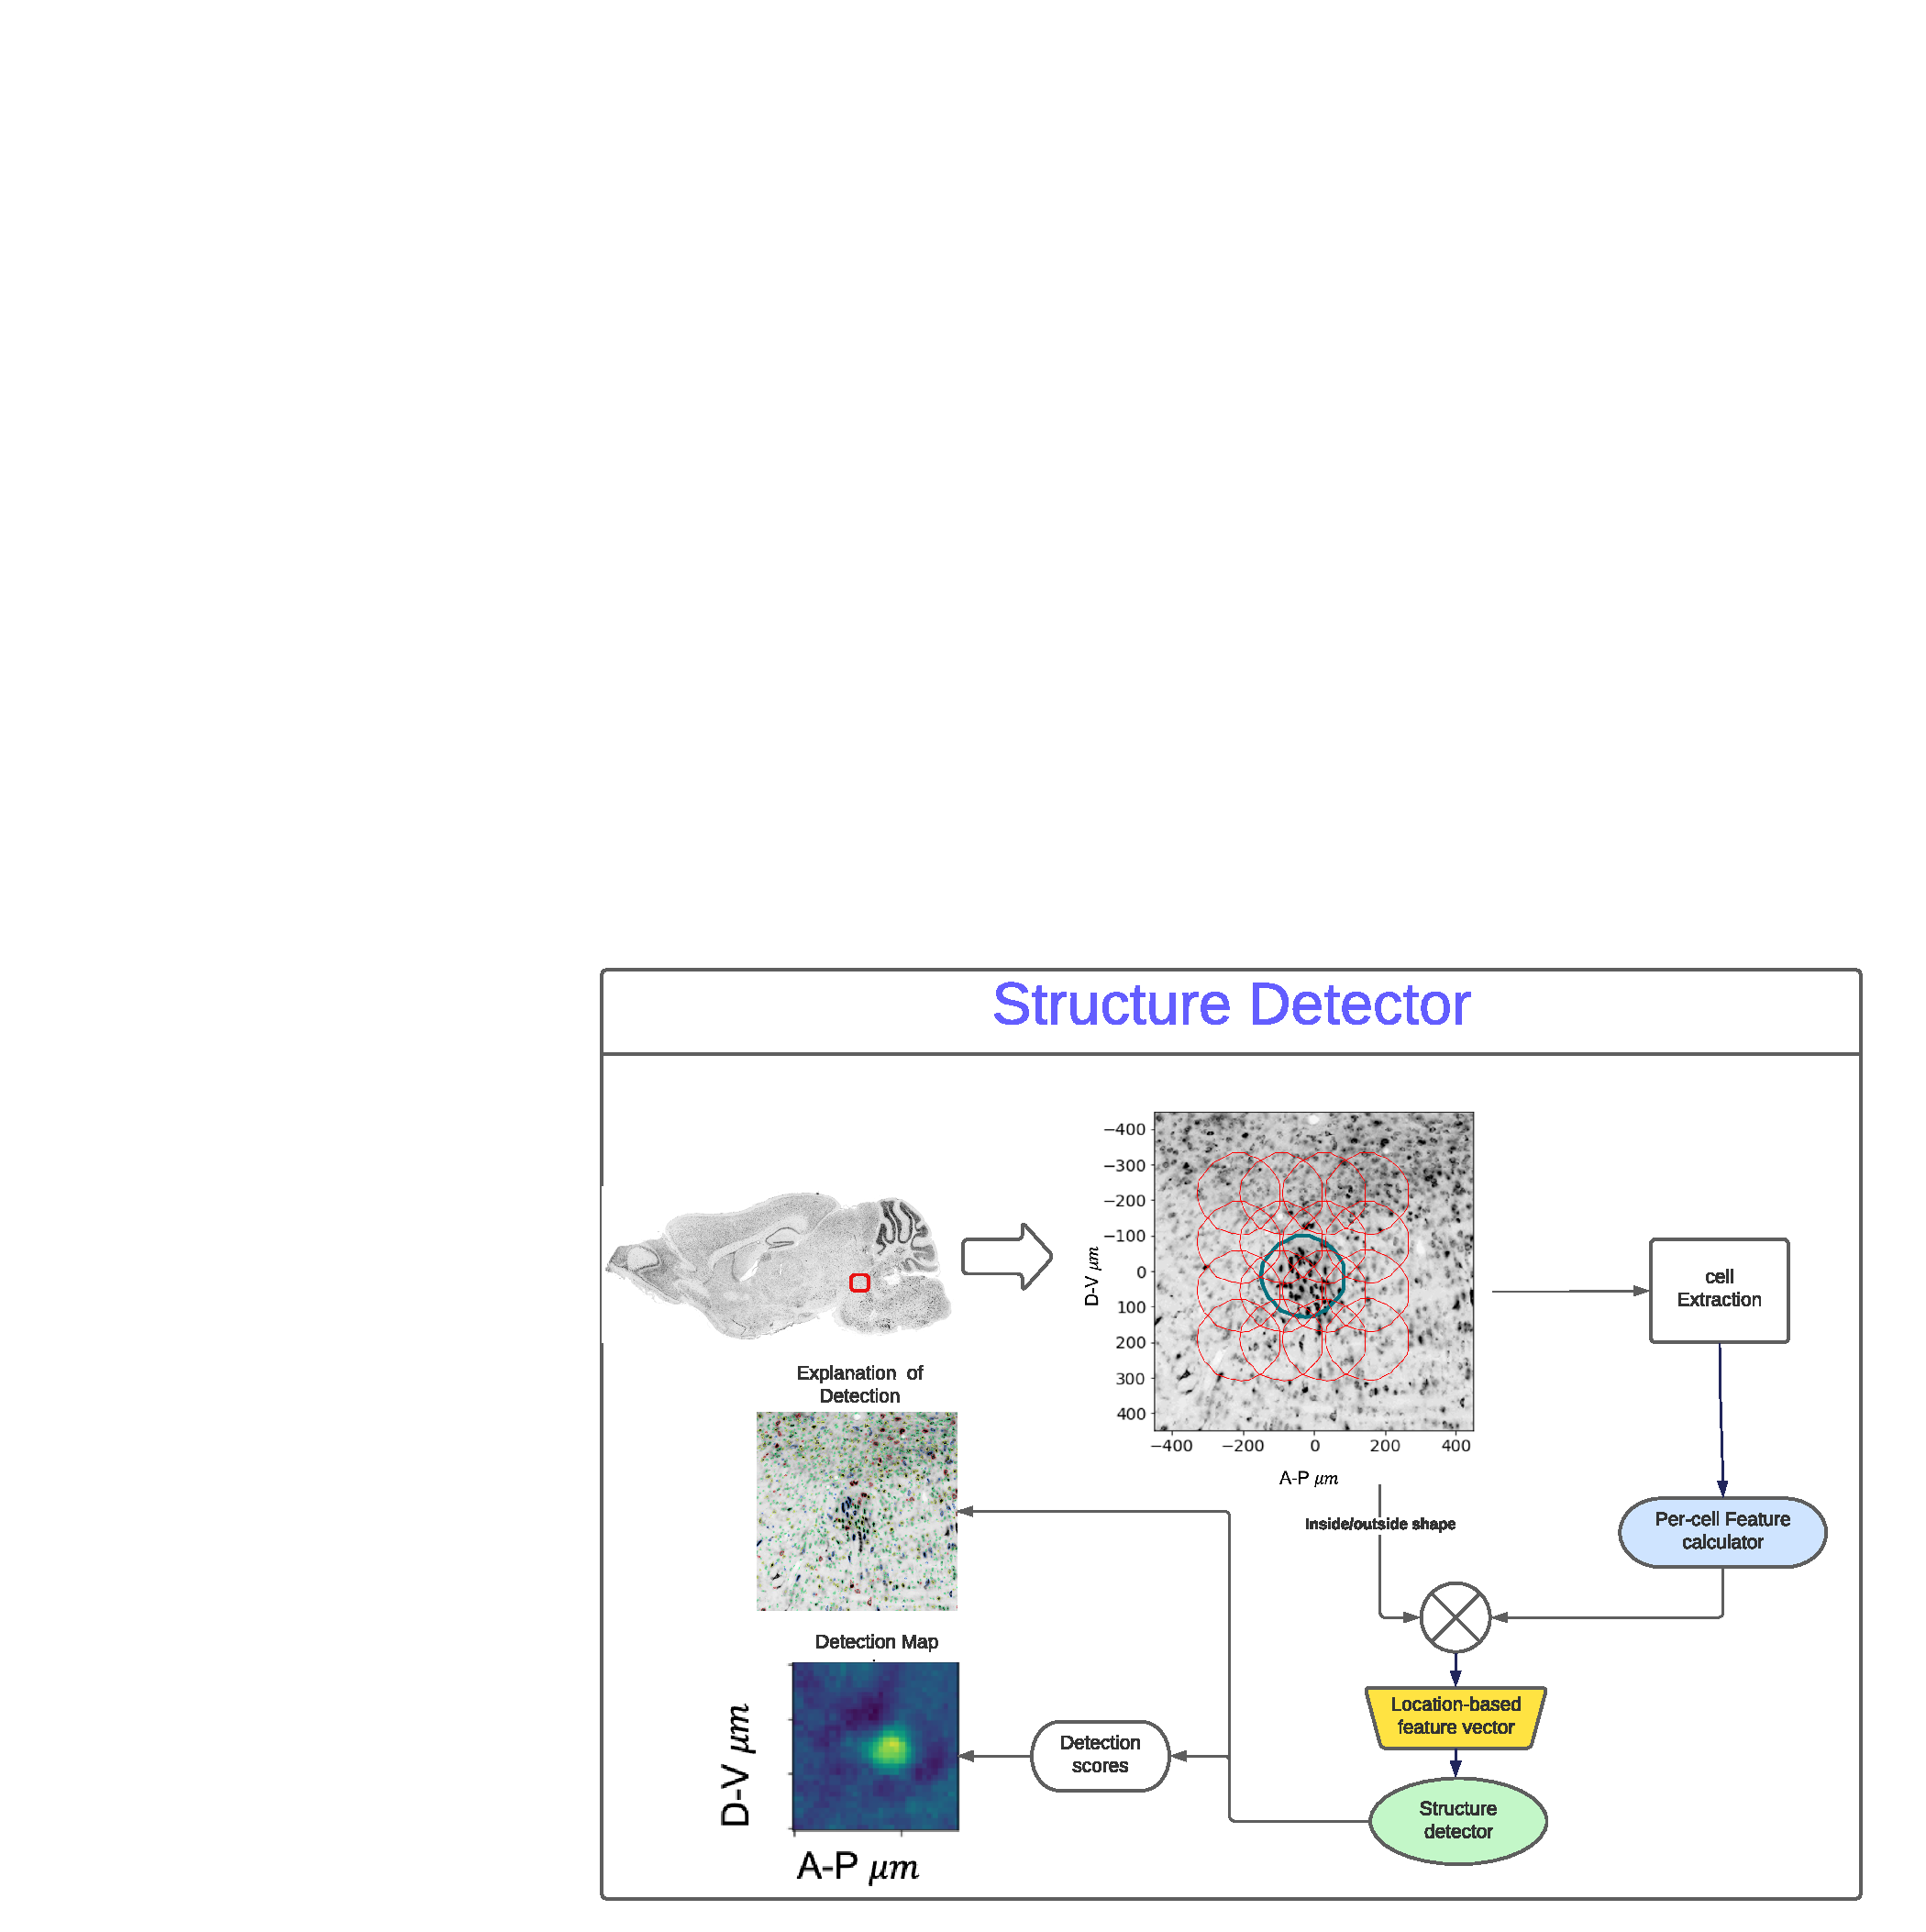
\includegraphics[width=\textwidth]{figures/detection.pdf}
  \caption{\label{fig:detector} {\bf Dataflow of the structure
      detector} (terms that are underlined are described in more
    detail in the methods section.) {\bf (a)} The input to the detector
    is a sequence of sections from a whole brain. The red square
    indicates the search area which is defined using rough
    alignment. {\bf (b)} the 3D shape of the structure is {\em
      extracted from manual annotations},
    shifting this shape defines which cells are in the structure and
    which are outside. {\bf (c)} The cells from the whole brain are
    extracted. {\bf (d)} For each extracted cell we compute a set of
    {\em shape descriptors}, forming the per-cell feature vector. {\bf (e)}
    The shifted shapes from step (b) partition the cells into those
    that are inside the structure and those that are close to the
    structure but outside it. {\bf (f)} using the features of these
    sets of cells a {\em region-based feature vector} is
    computed. {\bf (g)} the region-based feature vectors are passed
    through a {\em learned detection function} which outputs a
    detection score. {\bf (h)} the detection scores are organized in
    a {\em detection map}. From which two quantities are extracted:
    {\bf (i)} the detection location and {\bf (j)} the {\em detection
      confidence}. {\bf (k)} In addition, the system generates, based on the
    region feature vector and detection function, and {\em detection
      explanation}}
\end{figure}

\subsection{Detecting Structures}
The architecture of our structure detectors is described in
Figure~(\ref{fig:detector}). For each structure we have a separate
boundary shape, inferred from human annotations, and a learned
detection function that is learned from human annotations of the
location of the center of mass of the structures in particular
brains. The details of the learning process is described in the
methods section.

Detection is done in two steps. In the first, called ``rough
alignment'' we use an industry standard image based alignment method
to find approximate locations of the structures. The second step,
called the ``detection step'', is to apply each structure detector
at gridpoints every XX $\mu m$ up to distance of YY $\mu m $ from the
location of the rough detection. The result is a score map. Two
quantities are calculated from the score map: the most likely location
of the structure COM and the confidence level of the detection.

Figure~(\ref{fig:structureAccuracy}(a)) depicts the accuracy of the
detector, relative to a manual detection, for different confidence
levels. Figure (\ref{fig:structureAccuracy}(b)) compares the accuracy
of rough alignment to the accuracy of the detector. Note that most of
the detections are above the diagonal line, indicating that the
detections improve over the rough alignments. This trend is stronger
the higher the confidence level.

\begin{figure}[t]
  (a) \includegraphics[width=0.45\textwidth]{figures/ErrorVSconfidence.png}
  \hspace{1cm}
  (b)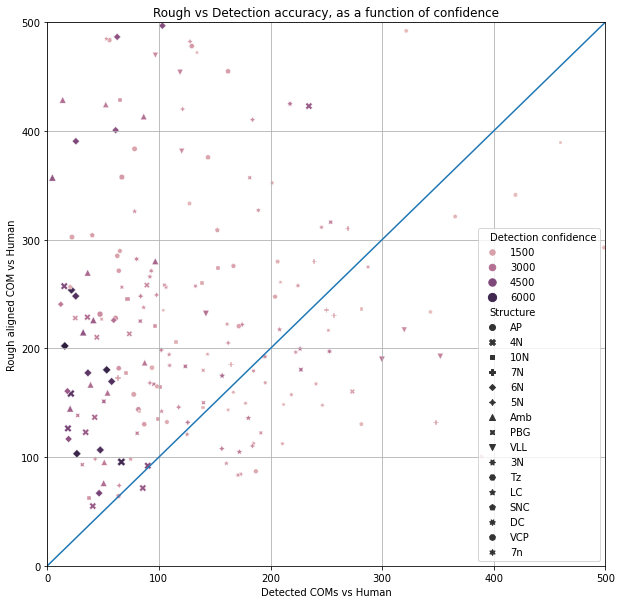
\includegraphics[width=0.45\textwidth]{figures/RoughVSdetection.png}
  \caption{\label{fig:structureAccuracy} {\bf Evaluation of detection
      accuracy:} {\bf (a)} shows the relationship between detection
    confidence and the detection error relative to human annotation.
    {\bf (b)} A comparison of the accuracy achieved by rough alignment
    to the accuracy achieved using a detector. Points above the
    diagonal line corresponds to structures for which the error of the
    detection is smaller.}
\end{figure}

\begin{figure}[t]
  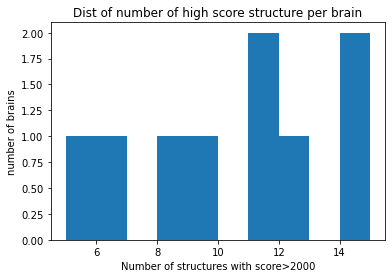
\includegraphics[width=0.4\textwidth]{figures/PerBrainStrongDetections.png}
  \caption{\label{fig:ConfidentStructureHist} {\bf Number of
      structures with detection confidence > 2000 per brain} is
    between 5 and 14 per brain. 5/9 brains have more than 10 confident detections.}
\end{figure}



\subsubsection{Explaining detections}
For each detection we generate an explanation. The explanation
consists of an annotated image in which cells that are typical of the
structure and cells that are typical of the region outside the
structure are highlighted. Figure~(\ref{fig:explaining}.)

\begin{figure}[t]
  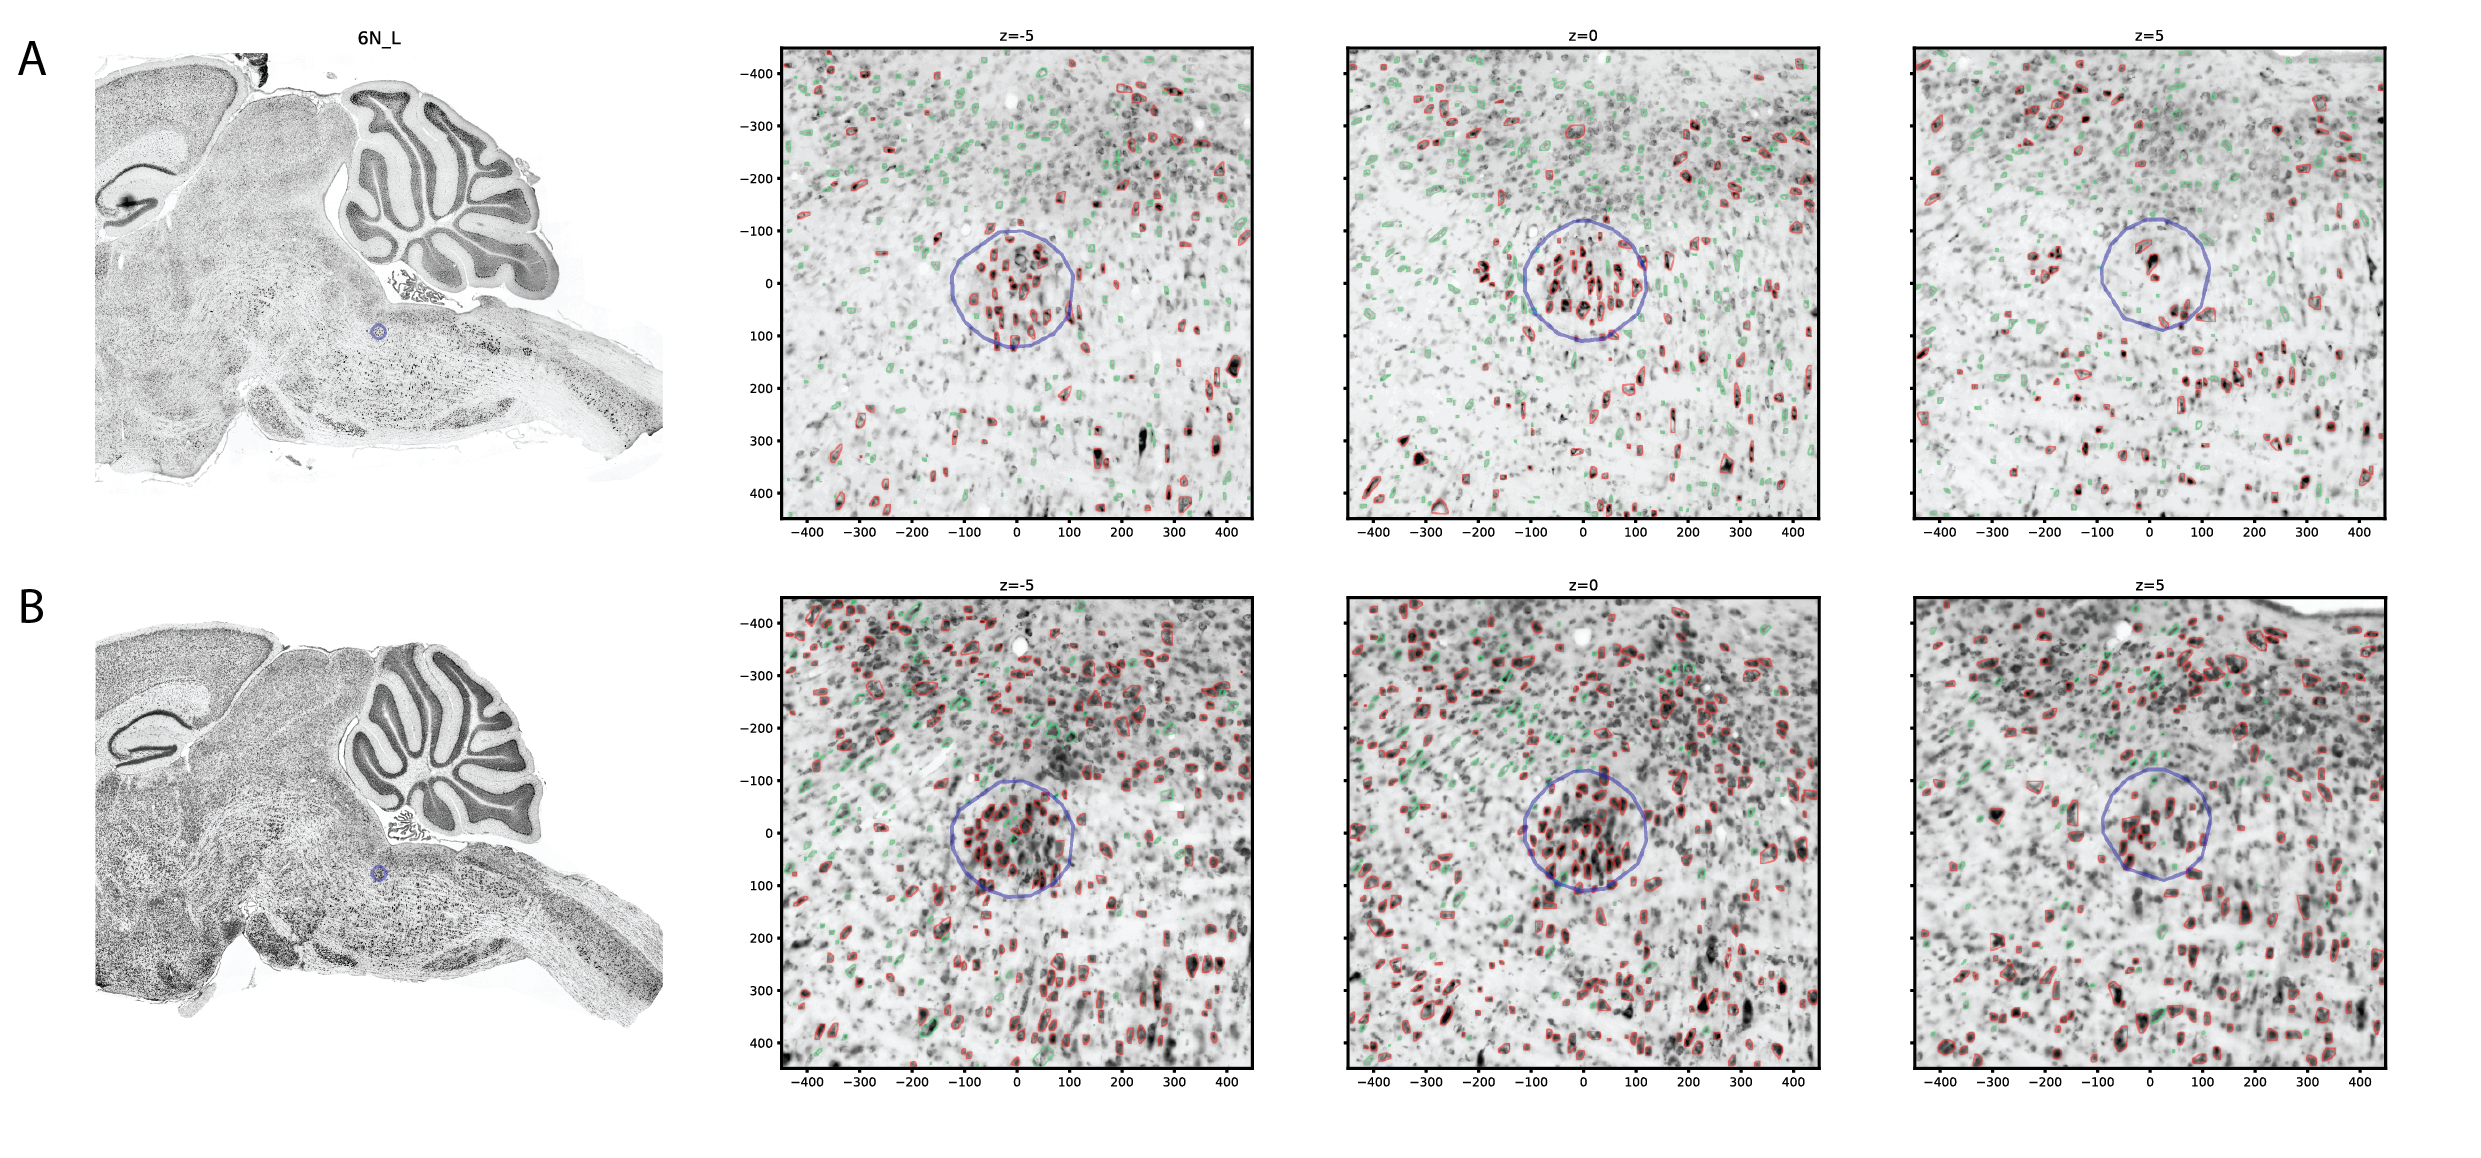
\includegraphics[width=\textwidth]{figures/DetectionExplanation.png}
  \caption{\label{fig:explaining} {\bf explaining detections:} visual explanations for the
    detection of 6N\_L in two brains. A and B are brain images of two
    brains at section z=0, marking the locations of 6N\_L with blue
    contours and showing cell distributions of the top 3 important
    features for regions inside and outside the contours.  The cells
    come from three sections, 100 microns apart. The red marked cells
    are evidence of the inside of the structure, the green cells,
    which are much smaller, are evidence of the outside. Note that
    section z=5 has very few cells. The detector overcomes this by
    combining information from all sections.  The bottom brain is
    stained darker than the top one, which is likely to confuse a
    method that is not cell based.}
  \end{figure}

\subsection{Detecting marked cells}

\begin{figure}[t]
  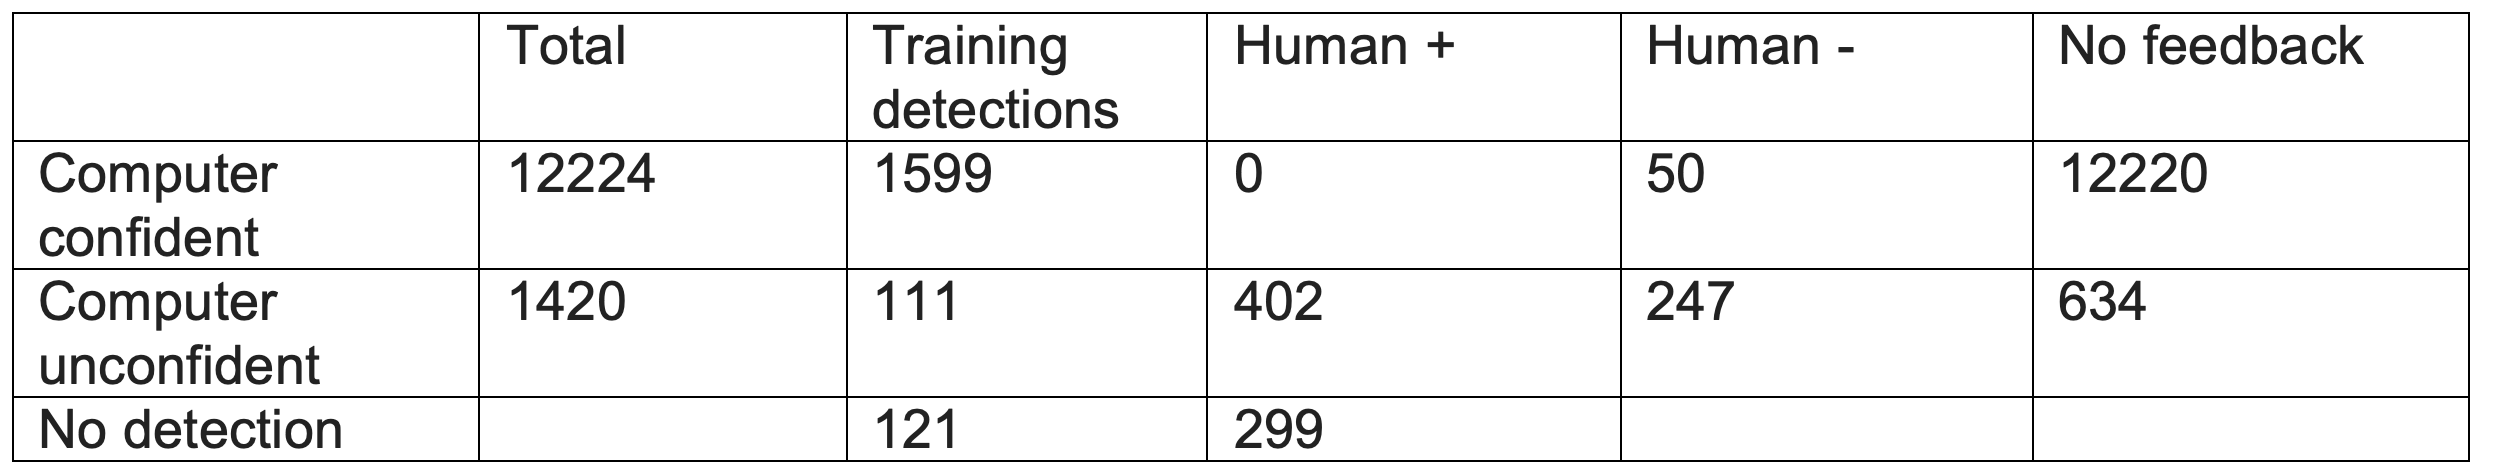
\includegraphics[width=\textwidth]{figures/MarkedCellsDetectionNumbers.png}
\end{figure}

\begin{figure}[b]
  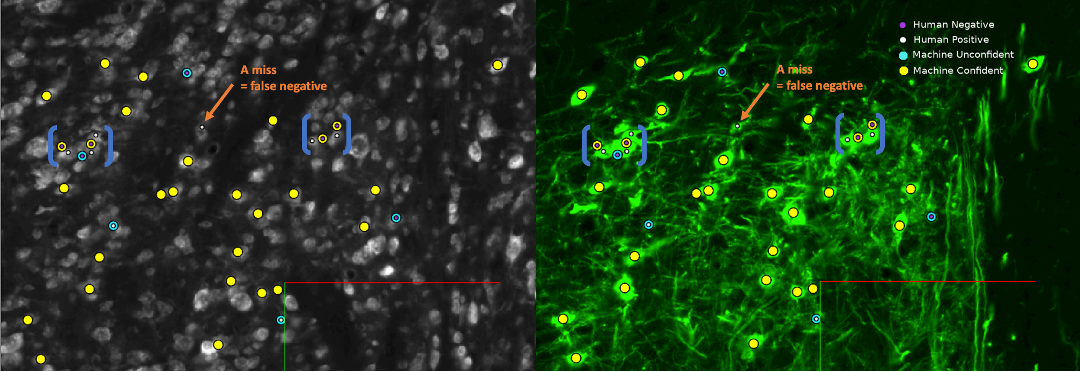
\includegraphics[width=\textwidth]{figures/Marked_cell_detections.png}
  \caption{}
\end{figure}

\iffalse
\begin{itemize}
\item The amount of manual work that it takes to manually mark cells.
\item inter-rater and intra-rater disagreement rate.
\item How to count false detections "with approximately correct
  detections detection".
\item How to quantify reduced mental load of QA vs detection.
\end{itemize}
\fi
\newpage

\section{Methods}

\subsection{Structure Detection}

\begin{figure}[t]
  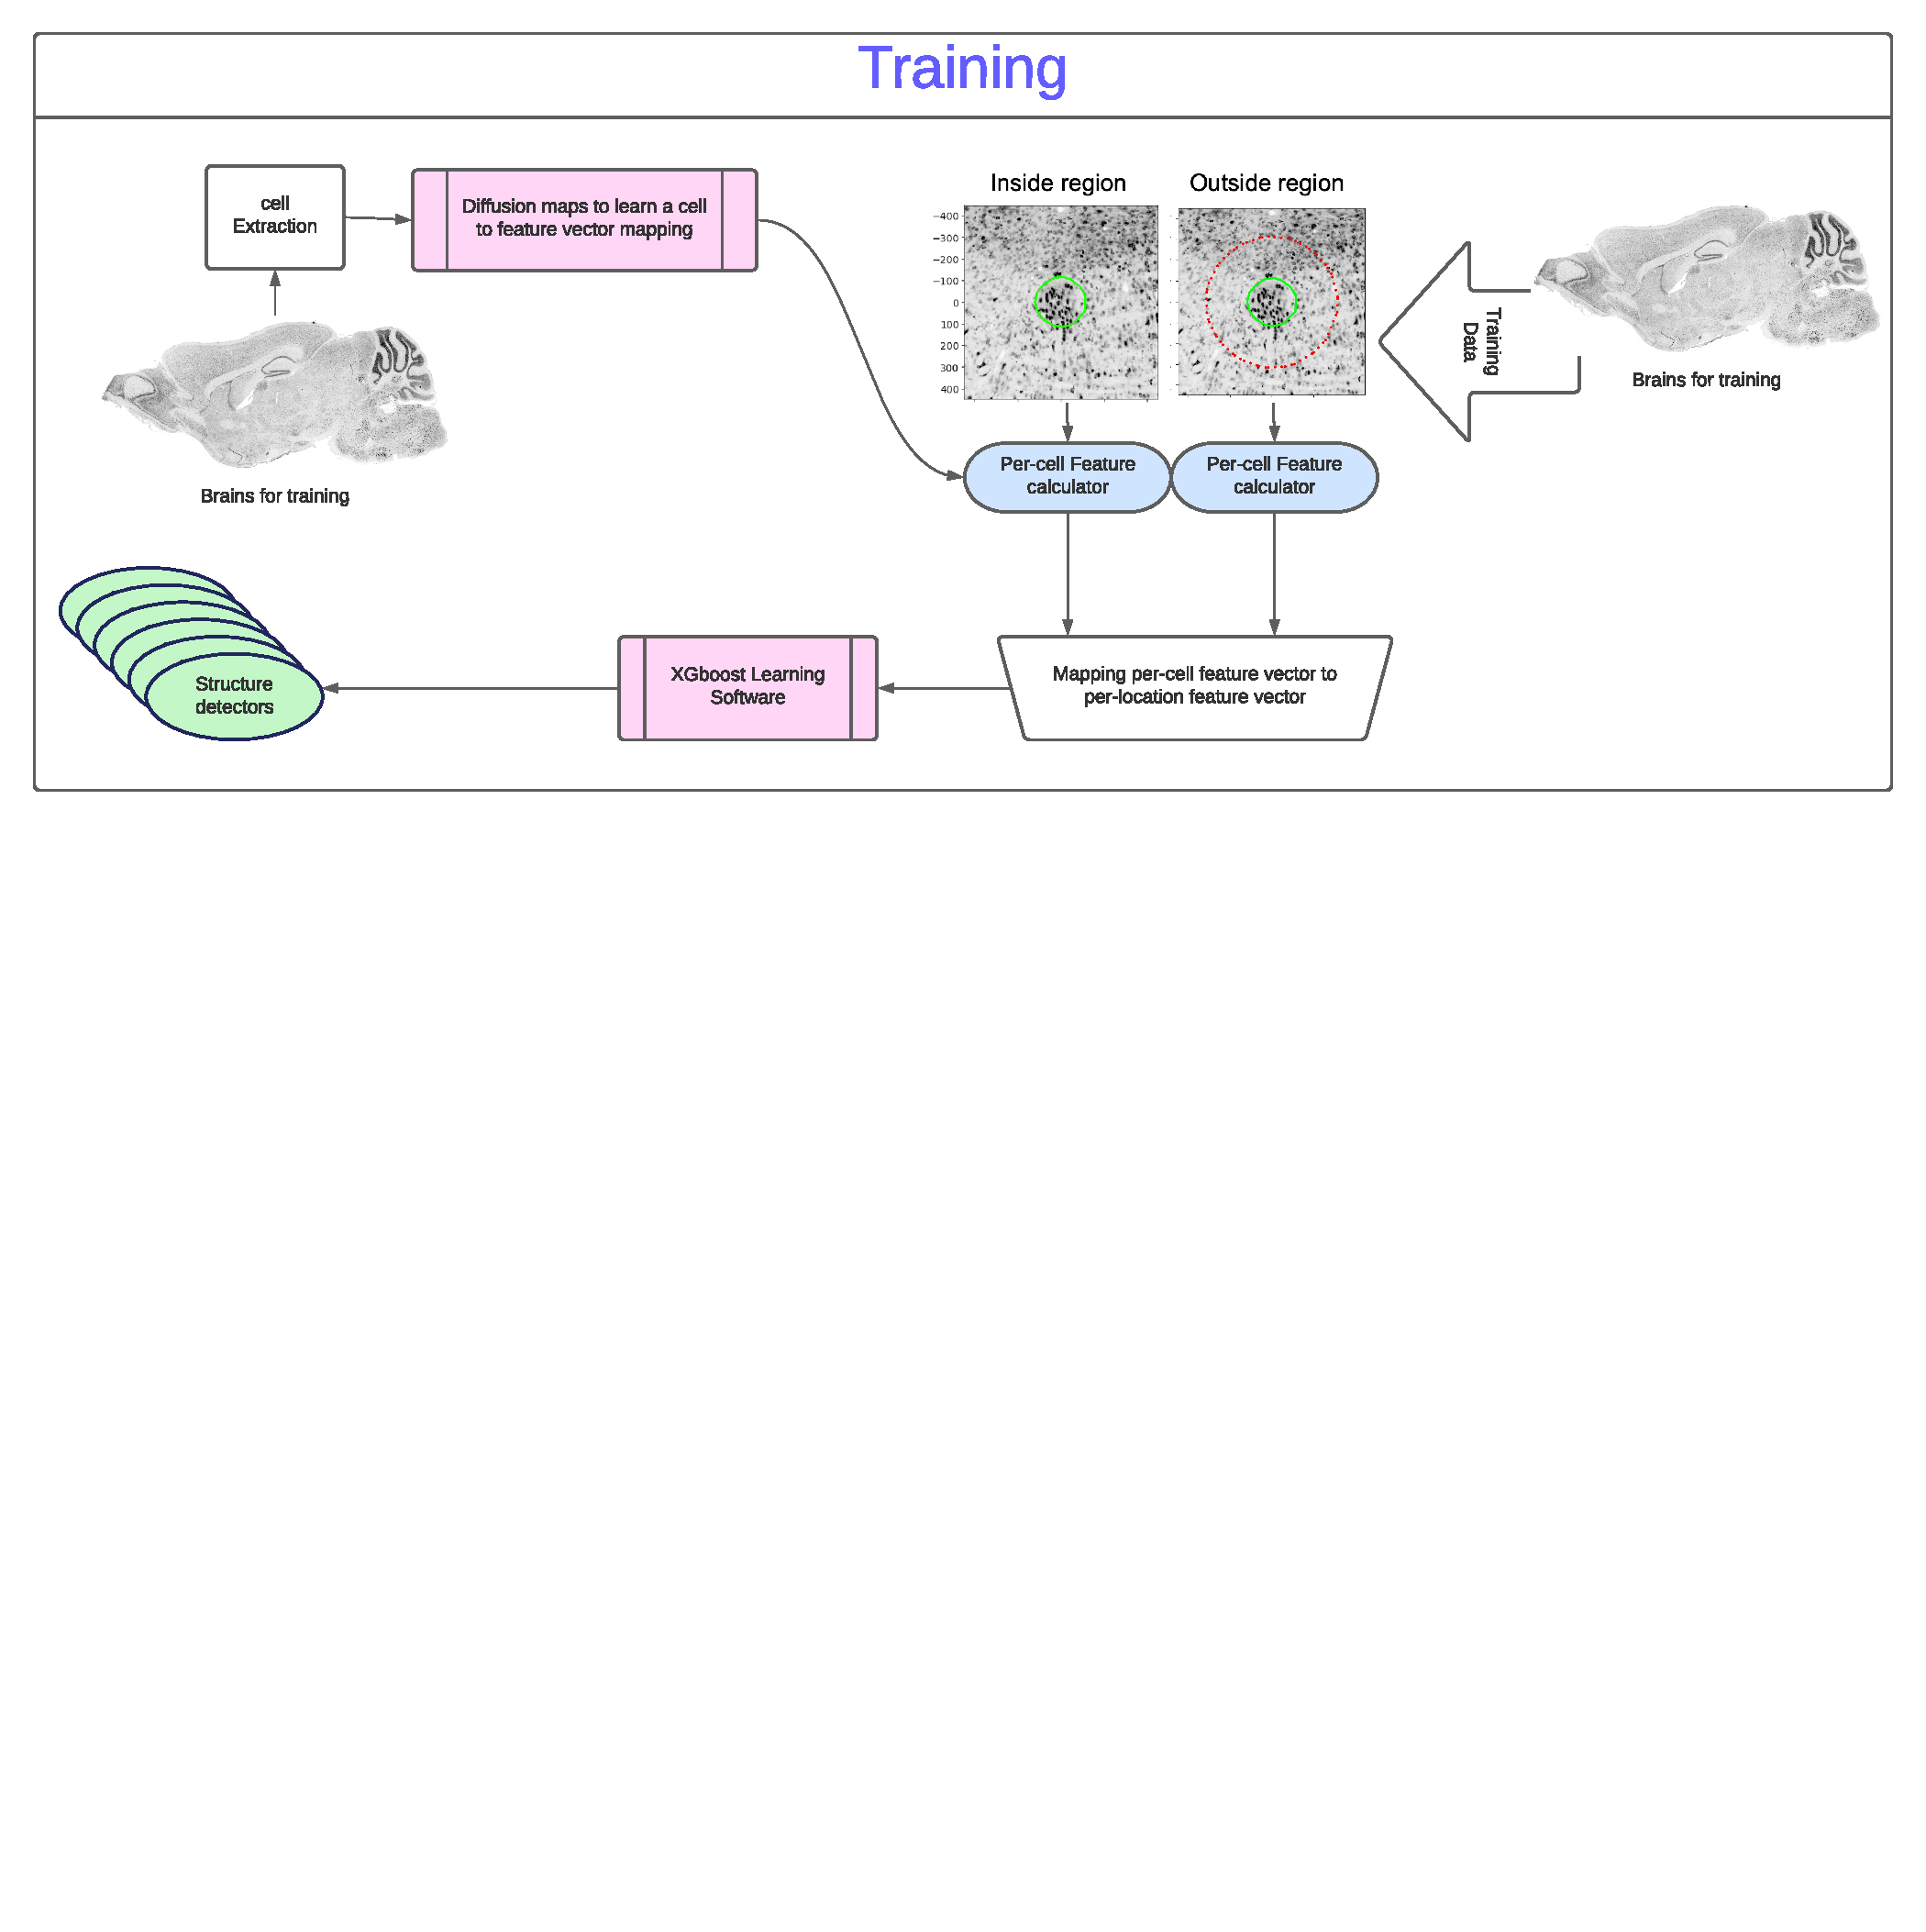
\includegraphics[width=\textwidth]{figures/Training.pdf}
  \caption{Training \label{fig:training}}
\end{figure}
The design of the structure detector system is described in Figure~\ref{fig:architecture}.
The system consists of two subsystems: the structure detector whose
function is to determine the location os brain structure, and the ML
subsystem which uses machine learning to create the structure detector.

The detectors combine three sources of information:
\begin{itemize}
    \item {\bf Images of aligned sections:} The Nissl images of XX brains are the primary information source. They are also by far the largest at XXX GB per brain.
    \item {\bf The Atlas} is a representation of the shape of each
      structure and the relative locations of the structures. The
      first step of the shape derivation was for three anatomists to
      annotate structures in three brains. This was a labor intensive
      step which took a total of XXX hours. The seccond step involved
      aligning the annotations from different brains to each other and
      taking the majority vote over the manual structures.
    \item {\bf COMs for individual brains:} For 10 brains we had an
      anatomist locate the the center-of-mass of 26-31 structures in 9
      brains.~\footnote{DK52 not included because it is used for the
        rough alignment}
\end{itemize}

Below we describe each component of the system:

\subsubsection{Cell based analysis}

Our system does not use the grey-values of the brain sections
directly, instad it uses the shapes of the cells. The main advantages
of this approach are (1) reduced sensitivity to changes in brightness
and contrast, and (2) the ability to provide meaningful explanations
for machine detections.

\paragraph{Cell extraction}
The goal of this step is to extract ``local cell configurations'',
those include neurons and glia cells. Both single cells and overlapping
or very close cells are included.

Cell extraction is performed using a locally adaptive threshold,
followed by normalization. The normalization is done using local
shift and scale operations whose result if that the local mean is 0
and the local std is 1. This is followed by thresholding the image at
value X and computing of connected components. Each connected
component is rotated so that it's long axis is vertical. The result
is a square image patch, typically of 50x50 pixels, together with the
angle of rotation of the long axis.

The quantification of the cell shapes uses a  combination of
pre-defined and adaptive features. 

\paragraph{Pre-defined cell-shape features}.
We use the Hu Moment features:

\paragraph{Adaptive Shape Features}
The Hu features are mathematically elegant and easy to
compute. However, they are not adapted to images of segmented cells.

To overcome this deficiancy we use an unsupervised learning algorithm
which generates a dimensionality reducing mapping from cell images to
a vector describing the shape. The dimensionality reducing method we
use is {\em Diffusion
  eigen-maps}~\cite{belkin2003,coifman2005geometric} which is a
non-linear dimensionality reduction method based on the eigen-decomposition
of the Laplace-Beltrami operator. Roughly speaking, it is a non-linear
generalization of Principal Component Analysis.

Figure~(\ref{fig:eigenmap}) shows that eigen-vectors identified by this method capture intuitive
properties of the cell shape such as size and roundness. In addition,
the method captures the short sequence  of glia cells (do these sequences
have a name?).

The eigen-vector representation is robust against brain to brain
variability as well as variability due to differences in imaging
modality.

\begin{figure}[t]
  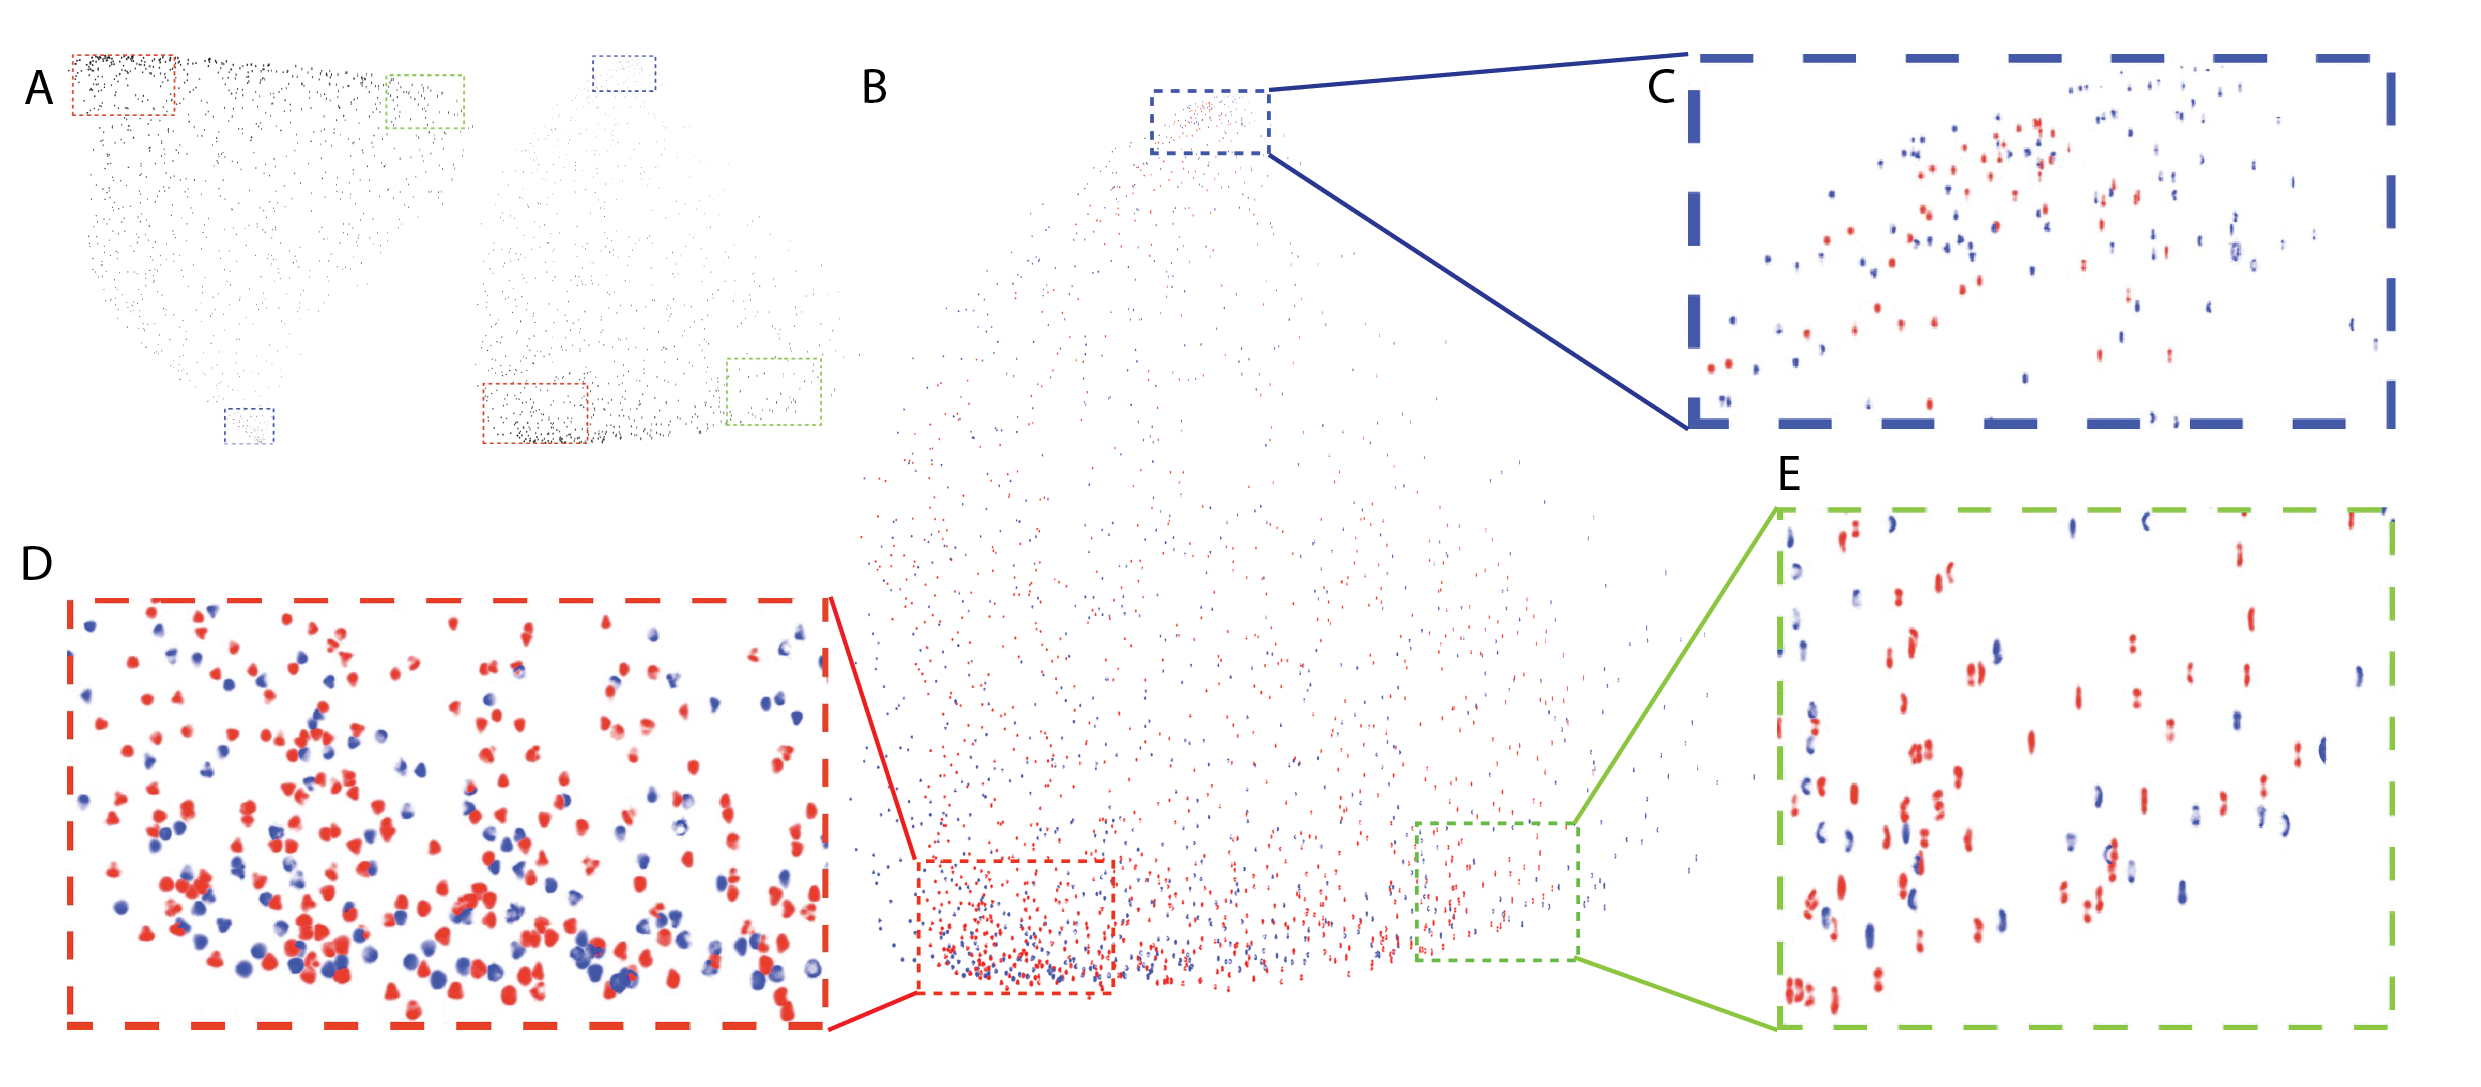
\includegraphics[width=\textwidth]{figures/Diffusionmap.png}
  \caption{\label{fig:eigenmap}{\bf Alignment of diffusion mappings:} A presents the
    similar original cell clouds in diffusion mappings of two brains
    using different modalities. After transformation, the two cell
    clouds matched well as shown in B. We marked the three corners of
    aligned mappings and gave details of these three regions in C, D
    and E.  }
\end{figure}

\paragraph{Location based feature vector} uses Difference between the CDFs for inside and outside of each structure (based on manually annotated structure boundaries). 
\paragraph{Detection functions} Combine the difference-of-CDF
features using boosted trees (XGBoost). Each structure has a
corresponding detector.

\paragraph{Structure detection confidence} The confidence of structure
  detections is measured by the prediction margin and by the sharpness
  of the detection peak.

\paragraph{ Structure detection explanation}

\section{DISCUSSION}

A challenge for extant methods \yoav{What are extant methods?} is the identification of brain structures. Classically, this relies on the use of a stain, i.e., a labels that marks a restricted part of the brain cells and allows both individual cells and clusters of like cells to be identified. In many cases the individual sections may carry distortions, and further need to be aligned to form a three-dimensional representation of a brain. Currently, human scanning is used to find the best match of a given structure, from the subject brain, to an annotated reference brain atlas. This match-to-sample approach does not readily support assessment of observational differences between laboratories nor provide a means for assessing and compensating for common systematic errors. An extended ML approach would support a mechanism for ML “self-annotation” of structures in sections. The output tag of a structure would be readily proof-read by human observation. Importantly, the curated set of output tags could serve as an objective set of fiducials. Fiducials are needed for alignment to other atlases, such as the Allen Atlas but there is no standardized method for fiducial selection.

This annotation allows tags cells to be placed into a common reference space so that the spatial distributions of functionally identified cells can be compared. This ML based tool supports detection of the 3d centroids of brain structures in serially sectioned counterstained mouse brains. The ML structure detectors essentially perform ML self-annotation of brain structures which can be used as fiducials for a more systematic registration of experimental brains into the widely accepted common reference space, the Allen Atlas. ML supported registration of brains to a common reference space, in turn allows co-display of ML labeled neuron data from different experimental brains.

A synergy of our ML cell and ML fiducial detection can support combining data  to common reference space. The ML detected labeled neurons are in the same brain stack as the ML detected landmarks and can be exported in a tethered fashion to new reference spaces. Thus our new algorithms provide assistance for the persistent challenge of combining connectomic data from different experimental brains into a common reference space. This will allow 3d comparisons of connectomic brain labeling data to help provide metrics for biological and for technical variability that underpins these studies. 

The central motivation of the work presented here is to develop tools to leverage human expertise rather than attempt to replace it; leveraging demands the use of ML methods that support meaningful confidence levels and can provide explanations for these confident predictions.



 \bibliographystyle{splncs04}
 \bibliography{Reference,bib}



\end{document}


